\documentclass[12pt]{article}
\usepackage{amsmath}
\usepackage{breakurl}
\usepackage[utf8]{inputenc}
\usepackage[titletoc,toc,title]{appendix}
\usepackage{float}
\usepackage{enumitem}
\usepackage{hyperref}

% images
\usepackage{graphicx}
\DeclareGraphicsExtensions{.pdf,.png,.jpg}
\graphicspath{ {./materials/} }

% listings
\usepackage{listings}
\usepackage[usenames,dvipsnames]{color}
\definecolor{listinggray}{gray}{0.9}
\definecolor{lbcolor}{rgb}{0.95,0.95,0.95}
\lstset{
backgroundcolor=\color{lbcolor},
    tabsize=4,    
%   rulecolor=,
    language=C,
        basicstyle=\scriptsize,
        aboveskip={1.5\baselineskip},
        columns=fixed,
        showstringspaces=false,
        extendedchars=false,
        breaklines=true,
        prebreak = \raisebox{0ex}[0ex][0ex]{\ensuremath{\hookleftarrow}},
        frame=single,
        numbers=left,
        showtabs=false,
        showspaces=false,
        showstringspaces=false,
        identifierstyle=\ttfamily,
        keywordstyle=\color[rgb]{0,0,1},
        commentstyle=\color[rgb]{0.026,0.112,0.095},
        stringstyle=\color[rgb]{0.627,0.126,0.941},
        numberstyle=\color[rgb]{0.205, 0.142, 0.73},
%        \lstdefinestyle{C++}{language=C++,style=numbers}’.
}
\lstset{
    backgroundcolor=\color{lbcolor},
    tabsize=4,
  language=C++,
  captionpos=b,
  tabsize=3,
  frame=lines,
  numbers=left,
  numberstyle=\tiny,
  numbersep=5pt,
  breaklines=true,
  showstringspaces=false,
  basicstyle=\footnotesize,
%  identifierstyle=\color{magenta},
  keywordstyle=\color[rgb]{0,0,1},
  commentstyle=\color{OliveGreen},
  stringstyle=\color{red}
  }

\title{Comparation of execution time sort algorithms implementations in C\\
Counting sort and Bucket sort}
\author{
	  Pelczar Piotr\\
	  \small{\texttt{piotpel817@student.polsl.pl}}
	}
\usepackage{datetime}
\newdate{date}{08}{03}{2014}
\date{\displaydate{date}}
 
\begin{document}
\maketitle
 
\begin{abstract}
This paper describes and compares counting sort and bucket sort algorithms implementations written in C language.
The main doubt is what is the impact of pointers operations in \emph{bucket sort} relatively to single operations on arrays
in \emph{counting sort}.
\end{abstract}

\renewcommand{\contentsname}{Contents}

\newpage
\tableofcontents

\newpage
\section{Introduction}
\label{sec:intro}

This paper describes computational complexity comparation of two sorting algorithms based on indexing keys: \emph{bucket sort} and \emph{counting sort}. This is specific class of algorithms, which implicts some constraints on sorting keys. Keys are indicies of arrays in implemetations so in special cases the key have to be positive whole number between 0 and max integer range (0..65536) depends on platform. Both algorithms have simmilar linear computational complexity.

Bucket sort creates array of one-way list of elements (a.k.a. \emph{buckets}), which is merged at the end. This behaviour requires pointer operations\cite{cormen}.

Counting sort creates an array that represents counts of keys, and next the prefix-sum is defined, which describes how many lower keys there are before each key\cite{cormen}. That allows to simply insert keys in proper place. Algorithm is stable\footnote{Positions of items are not relatively changed after algorithm iteration.}.

Both of algoritmhs has been implemented in C language.

This benchmark witch source code is avaliable on GitHub:\\
\url{https://github.com/athlan/polsl-benchmark-sort-algorithms}

\section{Implementation}
\subsection{Bucket sort}

Based on pseudocode\cite{czech}.

\lstinputlisting[language=C]{../code/sort_algorithms/bucket_sort.c}

\subsection{Counting sort}

Based on pseudocode\cite{czech}.

\lstinputlisting[language=C]{../code/sort_algorithms/counting_sort.c}

\section{Comparation}

\subsection{Methodology}

Codes has been compiled in gcc 4.2.1 compiler under MacOSX in 3 optimization modes (0 - none, 1, 2 and 3)\cite{man-gcc}.

\begin{lstlisting}
$ gcc -v
gcc version 4.2.1 (Apple Inc. build 5664)
\end{lstlisting}

Compilation process has been automated by Bash script listed in Appendix \ref{app:compilation}:

\begin{lstlisting}
$ ./bin/compile-all-optimizations.sh
\end{lstlisting}

The dataset is generated by script listed in Appendix \ref{app:dataset}. \emph{n} numbers (keys) are generated from range \emph{min} to \emph{max} which determines range of keys.

\begin{lstlisting}
$ ./bin/rand-dataset.sh min max n
\end{lstlisting}

The algorithms are invoked by benchmark program listed in Appendix \ref{app:benchmark} in \emph{n} iterations (n = 100). Memory allocations are not measured, time counters are aware only for sorting operations. The benchmark is fired by Bash script (Appendix \ref{benchmark-script}) with generates same dataset for each sorting and run all optimized compilations. The results are printed as friendly CSV format:

\begin{lstlisting}
$ ./bin/run-benchmark.sh > results.csv
\end{lstlisting}

\subsection{Hardware}

Benchmark has been done on MacBook Pro with 2.4GHz Intel with single phisical dual core processor:

\lstinputlisting[language=C]{./materials/computer-info.txt}

\subsection{Results}

The benchmark runs sorting algorithms 100 times for gcc compilations (optimizations levels\cite{man-gcc}: 0, 1, 2 and 3) for generated datasets:

\begin{itemize}[noitemsep]
  \item 0.1k items
  \item 1k items
  \item 10k items
  \item 100k items
\end{itemize}

Key ranges:

\begin{itemize}[noitemsep]
  \item 0 - 0.1k
  \item 0 - 1k
  \item 0 - 10k
  \item 0 - 65k\footnote{Note that kays are 16-bit integers, so max value is 65 536}
\end{itemize}

\subsubsection{Comparation of algorithms}

\begin{figure}[H]
    \centering
    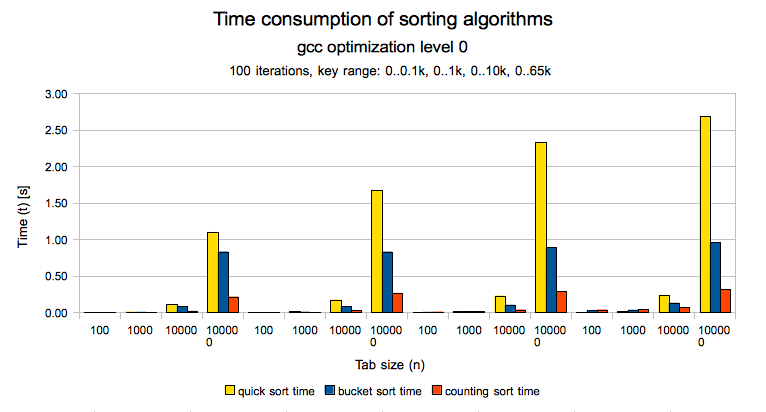
\includegraphics[width=1\textwidth]{compare-gcc-opt0}
\end{figure}

\begin{figure}[H]
    \centering
    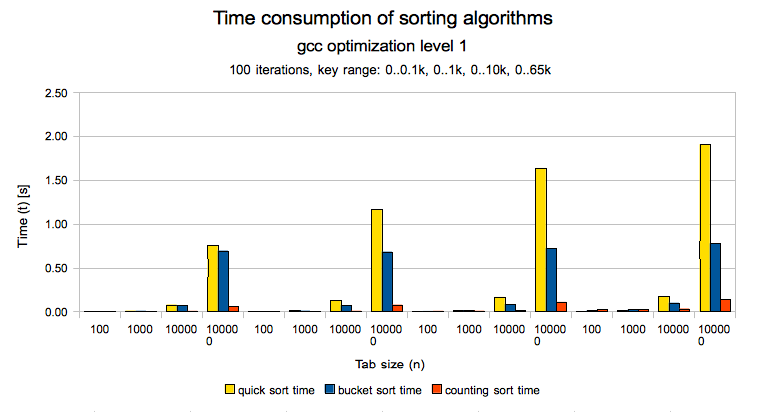
\includegraphics[width=1\textwidth]{compare-gcc-opt1}
\end{figure}

\begin{figure}[H]
    \centering
    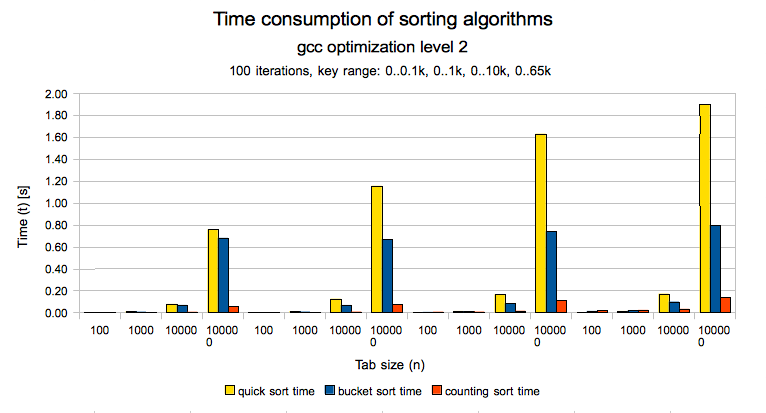
\includegraphics[width=1\textwidth]{compare-gcc-opt2}
\end{figure}

\begin{figure}[H]
    \centering
    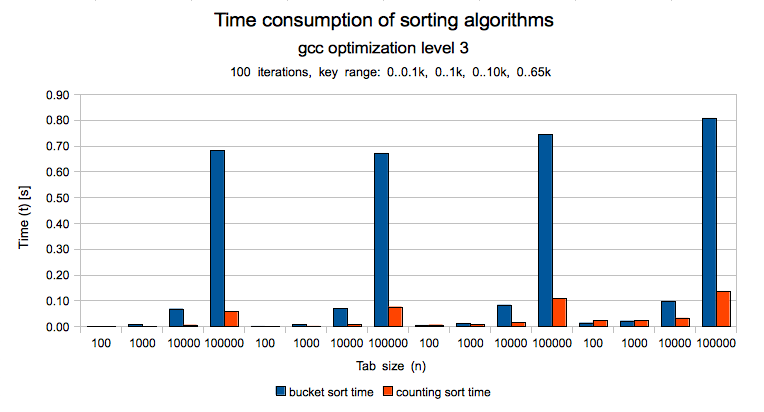
\includegraphics[width=1\textwidth]{compare-gcc-opt3}
\end{figure}

\subsubsection{Comparation of algorithms gcc optimized compilations}

\begin{figure}[H]
    \centering
    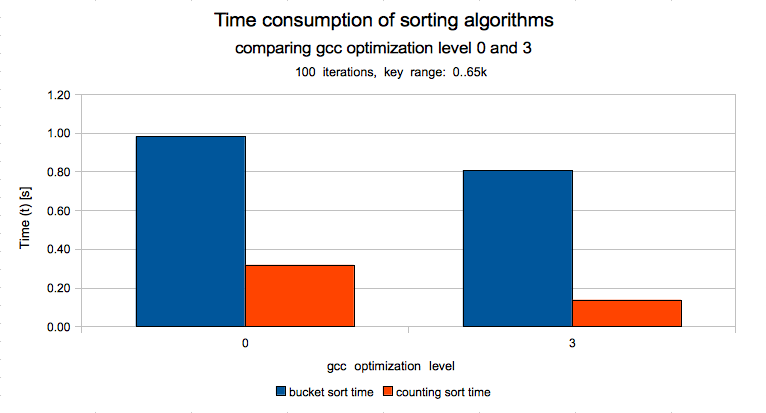
\includegraphics[width=1\textwidth]{compare-gcc-opt-0and3}
\end{figure}

\section{Conclusion}

\textbf{Counting sort is more effective than Bucket sort} (4.76 times in average and \textbf{5.91 times} for full optimization) in all cases for key range from 0 to 65k. Key range (in integer range) have no impact on time consumtion.

Moreover, \textbf{gcc optimization\footnote{3th level} have huge impact for Bucket sort which has operations on pointers} (132\% faster) and small impact for Counting sort (22\% faster).

Operations on pointers can be strongly optimized and have huge impact on algorithms.

\newpage
\begin{thebibliography}{9}
\addcontentsline{toc}{section}{References}

\bibitem{cormen}
  Thomas H. Cormen,
  \emph{Introduction To Algorithms}.
  The MIT Press,
  2nd Edition,
  2003.

\bibitem{czech}
  Zbigniew J. Czech,
  \emph{Algorytmy i struktury danych - Materiały dydaktyczne}.
  Politechnika Slaska, Instytut Informatyki,
  2011.
  ftp://sun.aei.polsl.pl/pub/zjc/asd.pdf [\emph{Retreived on 2013-03-08}]

\bibitem{man-gcc}
  gcc manual,
  http://linux.die.net/man/1/gcc

\end{thebibliography}

\begin{appendices}
	\section{Dataset generation script}
	\label{app:dataset}

	\lstinputlisting[language=Bash]{../bin/rand-dataset.sh}
	
	\section{Benchmark program}
	\label{app:benchmark}

	\lstinputlisting[language=C]{../code/benchmark.c}
	
	\section{Benchmark script}
	\label{app:benchmark-script}

	\lstinputlisting[language=Bash]{../bin/run-benchmark.sh}
	
	\section{Compilation script}
	\label{app:compilation}

	\lstinputlisting[language=Bash]{../bin/compile-all-optimizations.sh}

\end{appendices}

\end{document}